\chapter{Stadi di Uscita}

%--------------------------------------------------------------------------------------------

Per quanto rigurarda gli stadi di uscita, si collega in serie un filtro passa-basso attivo,
che avrà anche lo scopo di isolare l'assorbimento di corrente dai circuiti che generano i
segnali.

\begin{figure}[H]
    \centering
    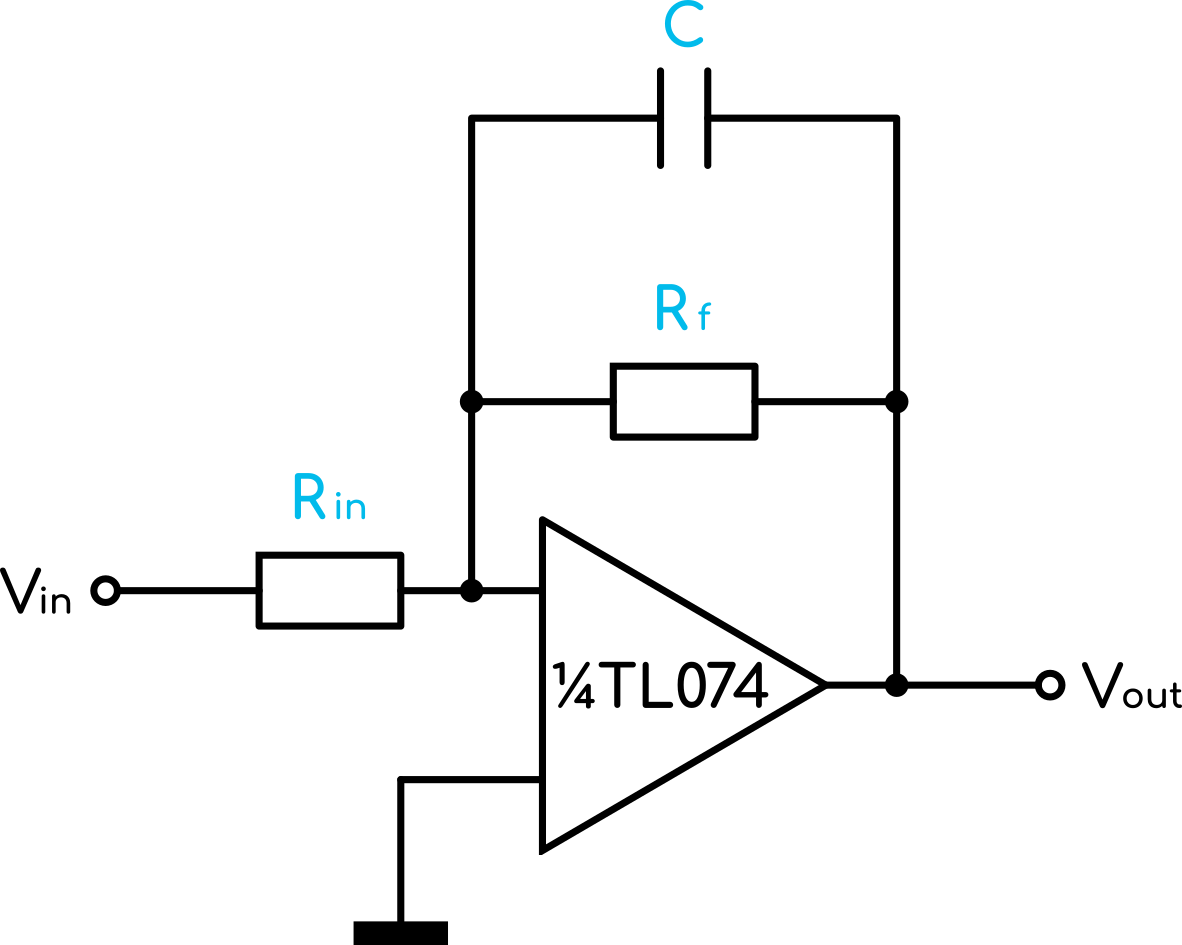
\includegraphics{circuits/active_filter_circuit.png}
    \caption{Circuito del filtro attivo utilizzato}
    \label{active_filter_circuit}
\end{figure}

sfruttando questa soluzione circuitale infatti, tutta la corrente prelevata dal circuito in
uscita verrà fornita dagli amplificatori operazionali. Le relazioni del circuito sono le
seguenti:

\begin{equation}\label{active_filter}
    V_{out}=-V_{in}\frac{R_f}{R_{in}}\cdot\frac{1}{1+j\omega R_fC}\ [V]
\end{equation}

\begin{equation}\label{fcut}
    f_{cut}=\frac{1}{2\pi R_fC}\ [Hz]
\end{equation}

\begin{equation}\label{gain1}
    A_{dB}=20log_{10}\left(\left|\frac{R_f}{R_{in}}\cdot\frac{1}{1+j\omega R_fC}\right|\right)\ [dB]
\end{equation}

oppure, dai valori misurati:

\begin{equation}\label{gain2}
    A_{dB}=20log_{10}\left(\frac{V_{rms\_out}}{V_{rms\_in}}\right)\ [dB]
\end{equation}

La frequenza di taglio viene presa attorno ai $30\ kHz$ per conservare tutto lo spettro audio
e rimuovere invece disturbi in alta frequenza dovuti ad esempio ai segnali di clock.
Scegliendo $R_f=100\ k\Omega$ quindi, il valore del condensatore va preso di circa $47\ pF$,
mentre $R_{in}$ deve avere valore pari a $R_f$. In questo modo si ottiene guadagno unitario e

\begin{equation}
    f_{cut}=\frac{1}{2\pi\cdot100\cdot10^3\cdot47\cdot10^-12}\approx34\ kHz
\end{equation}

Il setup di misura viene riportato in figura \ref{mis_filter}. Per la verifica del funzionamento
si misura il $V_{rms}$ di un segnale sinusoidale in ingresso e in uscita al filtro, agendo
sulla frequenza del suddetto segnale.

\begin{figure}[H]
    \centering
    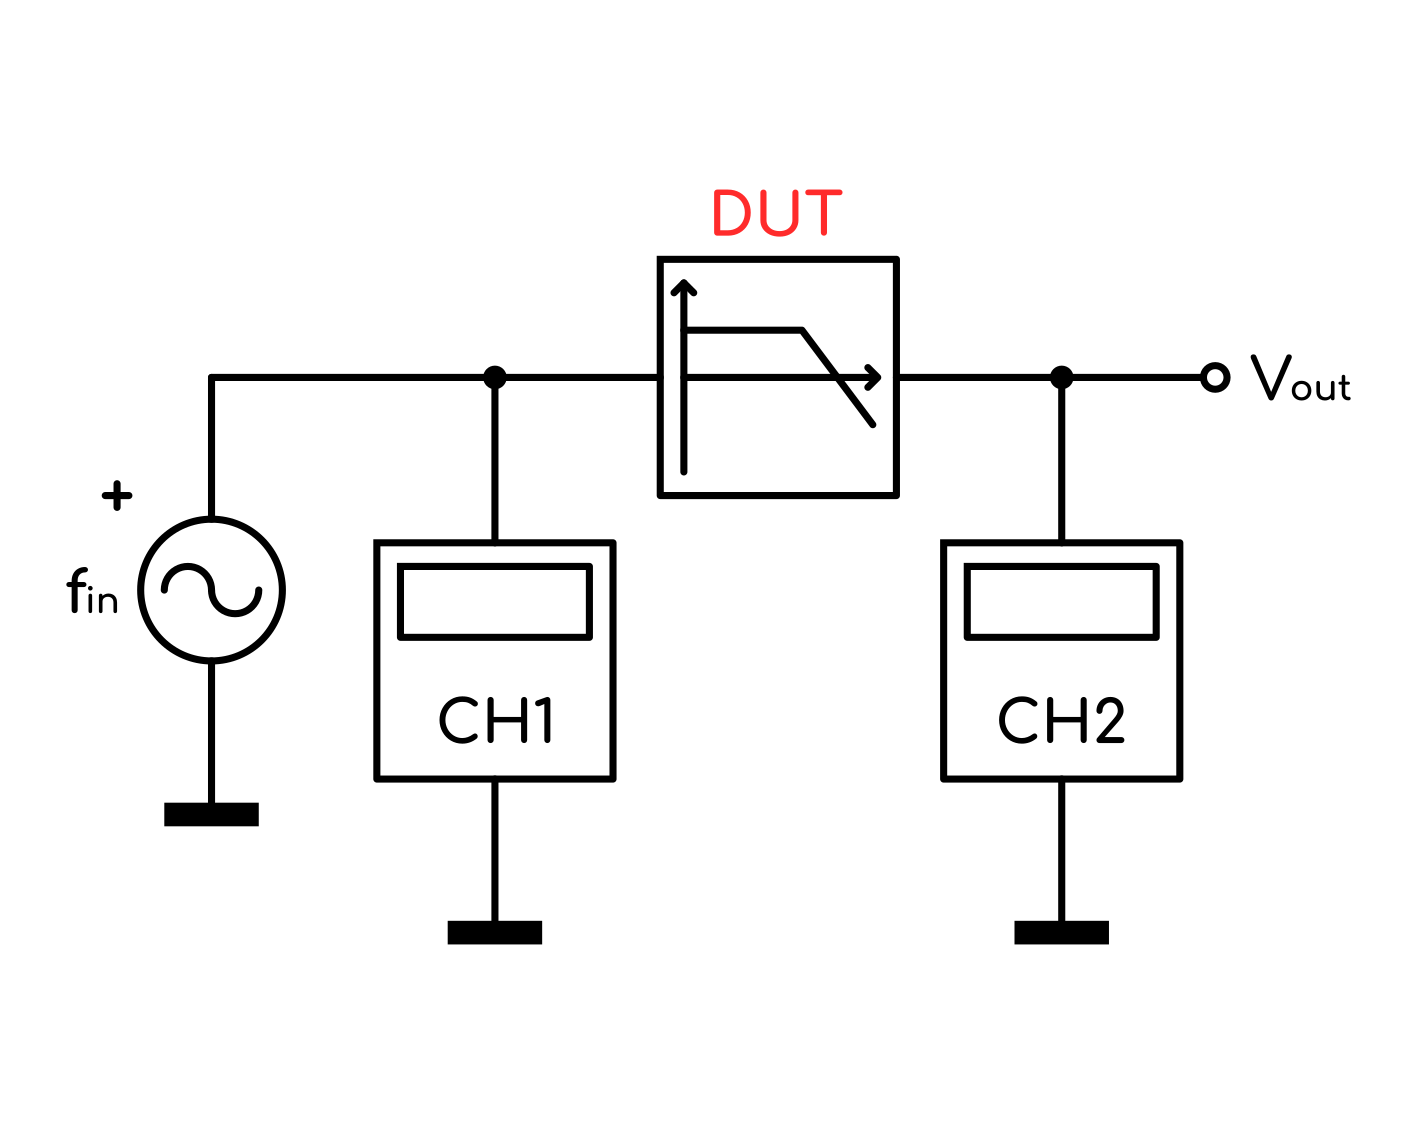
\includegraphics{block_diagrams/mis_filter.png}
    \caption{Setup di misura}
    \label{mis_filter}
\end{figure}

Successivamente, con la formula \ref{gain2} si calcola il valore del guadagno. Infine i dati
vengono raccolti in tabella, riportati in grafico e confrontati con i valori teorici calcolati
con la formula \ref{gain1}.

\begin{table}[H]
    \centering
    \csvreader[
    tabular = |C|C||C|L|,
    table head = {\hline \rowcolor{myLightGrey} $f_{in}\ [kHz]$ & $V_{rmsin}\ [V]$ & $V_{rmsout}\ [V]$ & $A_{dB}\ [dB]$\\\hline},
    late after line = \\\hline,
    ]{data/misure_bode.csv}{}{
    \csvcoli & \csvcolii & \csvcoliii & \csvcolv
    }
    \caption{Misure del guadagno del filtro attivo}
    \label{filter_table}
\end{table}

\begin{figure}[H]
    \centering
    \begin{tikzpicture}
        \centering
        \begin{semilogxaxis}[
                title = Diagramma di bode del filtro,
                no marks,
                width = 0.95\textwidth,
                height = 0.45\textwidth,
                xmin = 0.1, xmax = 4000,
                ymin = -40, ymax = 5,
                grid = major,
                grid style = {dashed, gray!30},
                xlabel = $f_{in}$,
                ylabel = $A_{dB}$,
                x unit = \si{\kHz}, y unit = \si{\dB},
                legend style = {at = {(0.5, -0.25)}, anchor = north},
                cycle list name = modular,
            ]

            \addplot
            table[x = fin, y = A dB calcolato, col sep = comma]{./data/misure_bode.csv};

            \addplot
            table[x = fin, y = A dB misurato, col sep = comma]{./data/misure_bode.csv};

            \legend{Formula \ref{gain1}, Formula \ref{gain2} (con i valori misurati)}
        \end{semilogxaxis}
    \end{tikzpicture}
\end{figure}

\begin{figure}[H]
    \centering

    \begin{subfigure}{.5\textwidth}
        \centering
        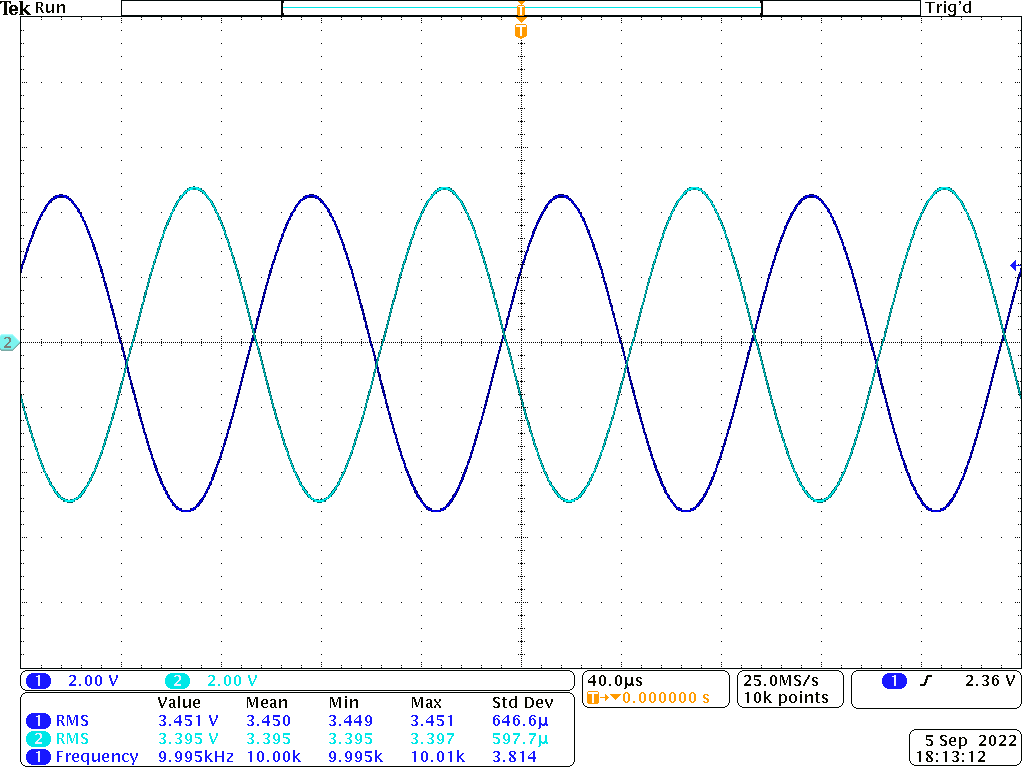
\includegraphics[scale = 0.2]{acquisitions/filter_10kHz.png}
        \caption{$f_{in}=10\ kHz$}
        \label{acq_filter_10kHz}
    \end{subfigure}%
    \begin{subfigure}{.5\textwidth}
        \centering
        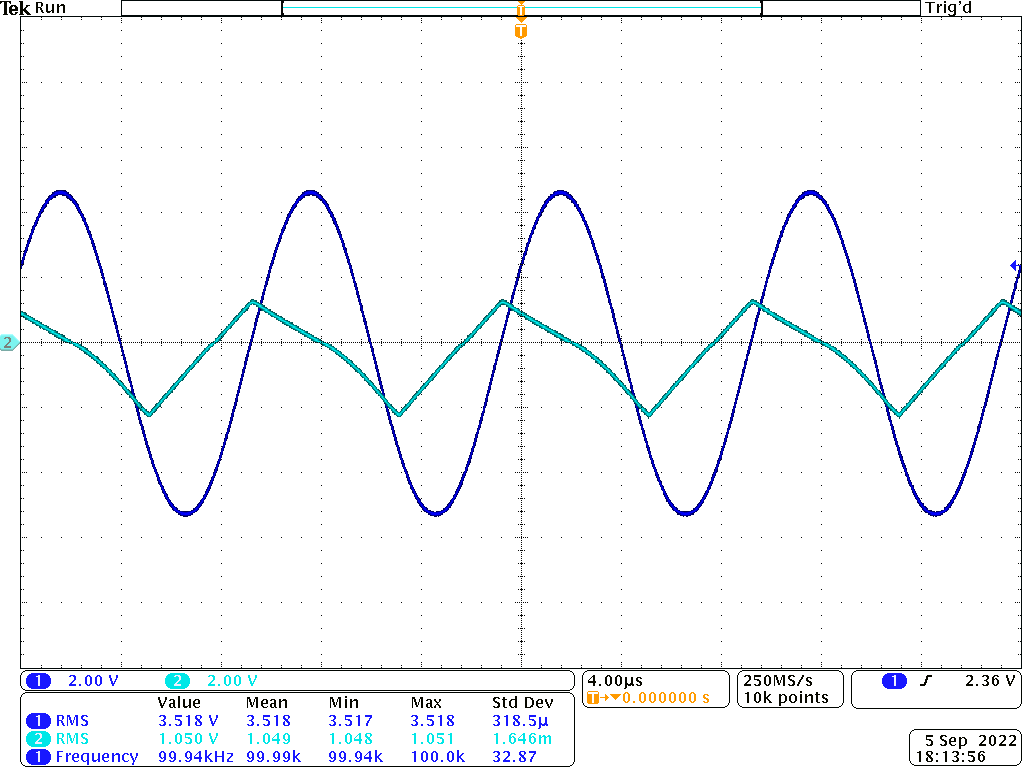
\includegraphics[scale = 0.2]{acquisitions/filter_100kHz.png}
        \caption{$f_{in}=100\ kHz$}
        \label{acq_filter_100kHz}
    \end{subfigure}
    \begin{subfigure}{.5\textwidth}
        \centering
        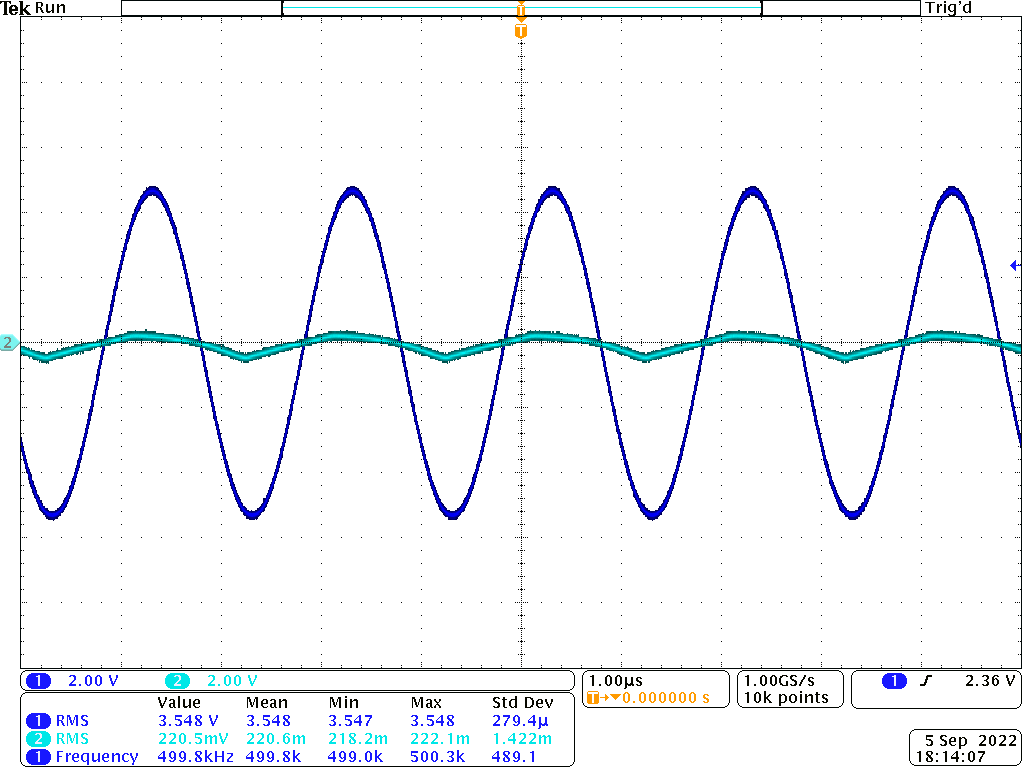
\includegraphics[scale = 0.2]{acquisitions/filter_500kHz.png}
        \caption{$f_{in}=500\ kHz$}
        \label{acq_filter_500kHz}
    \end{subfigure}%
    \begin{subfigure}{.5\textwidth}
        \centering
        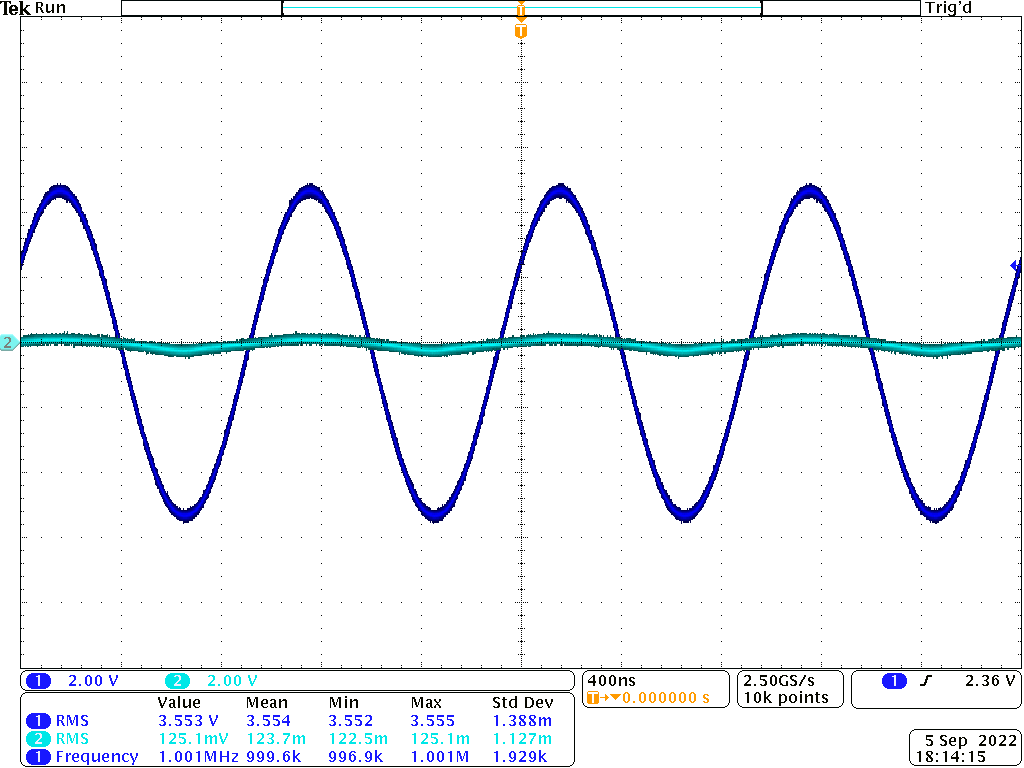
\includegraphics[scale = 0.2]{acquisitions/filter_1MHz.png}
        \caption{$f_{in}=1\ MHz$}
        \label{acq_filter_MHz}
    \end{subfigure}

    \caption{Acquisizioni dei segnali in ingresso e uscita al filtro per diversi valori di $f_{in}$}
    \label{acq_filter}
\end{figure}

In serie ai filtri per le onde a rampa e dente di sega viene anche collegato un amplificatore
invertente con guadagno unitario, con schema uguale a quello rappresentato in figura \ref{inverting_amp_circuit}
per riportare le onde alla loro forma originale, in quanto non sono simmetriche, come lo sono
invece le altre 3.

Infine, in serie a tutte le uscite degli ultimi operazionali prima del connettore, si collegano
dei potenziometri per la regolazione del volume e delle resistenze di protezione, dal valore
di circa $1\ k\Omega$ per limitare la corrente in uscita in caso di eventuali cortocircuiti,
che potrebbero provocare danni agli amplificatori operazionali.

\begin{figure}[H]
    \centering

    \begin{subfigure}{\textwidth}
        \centering
        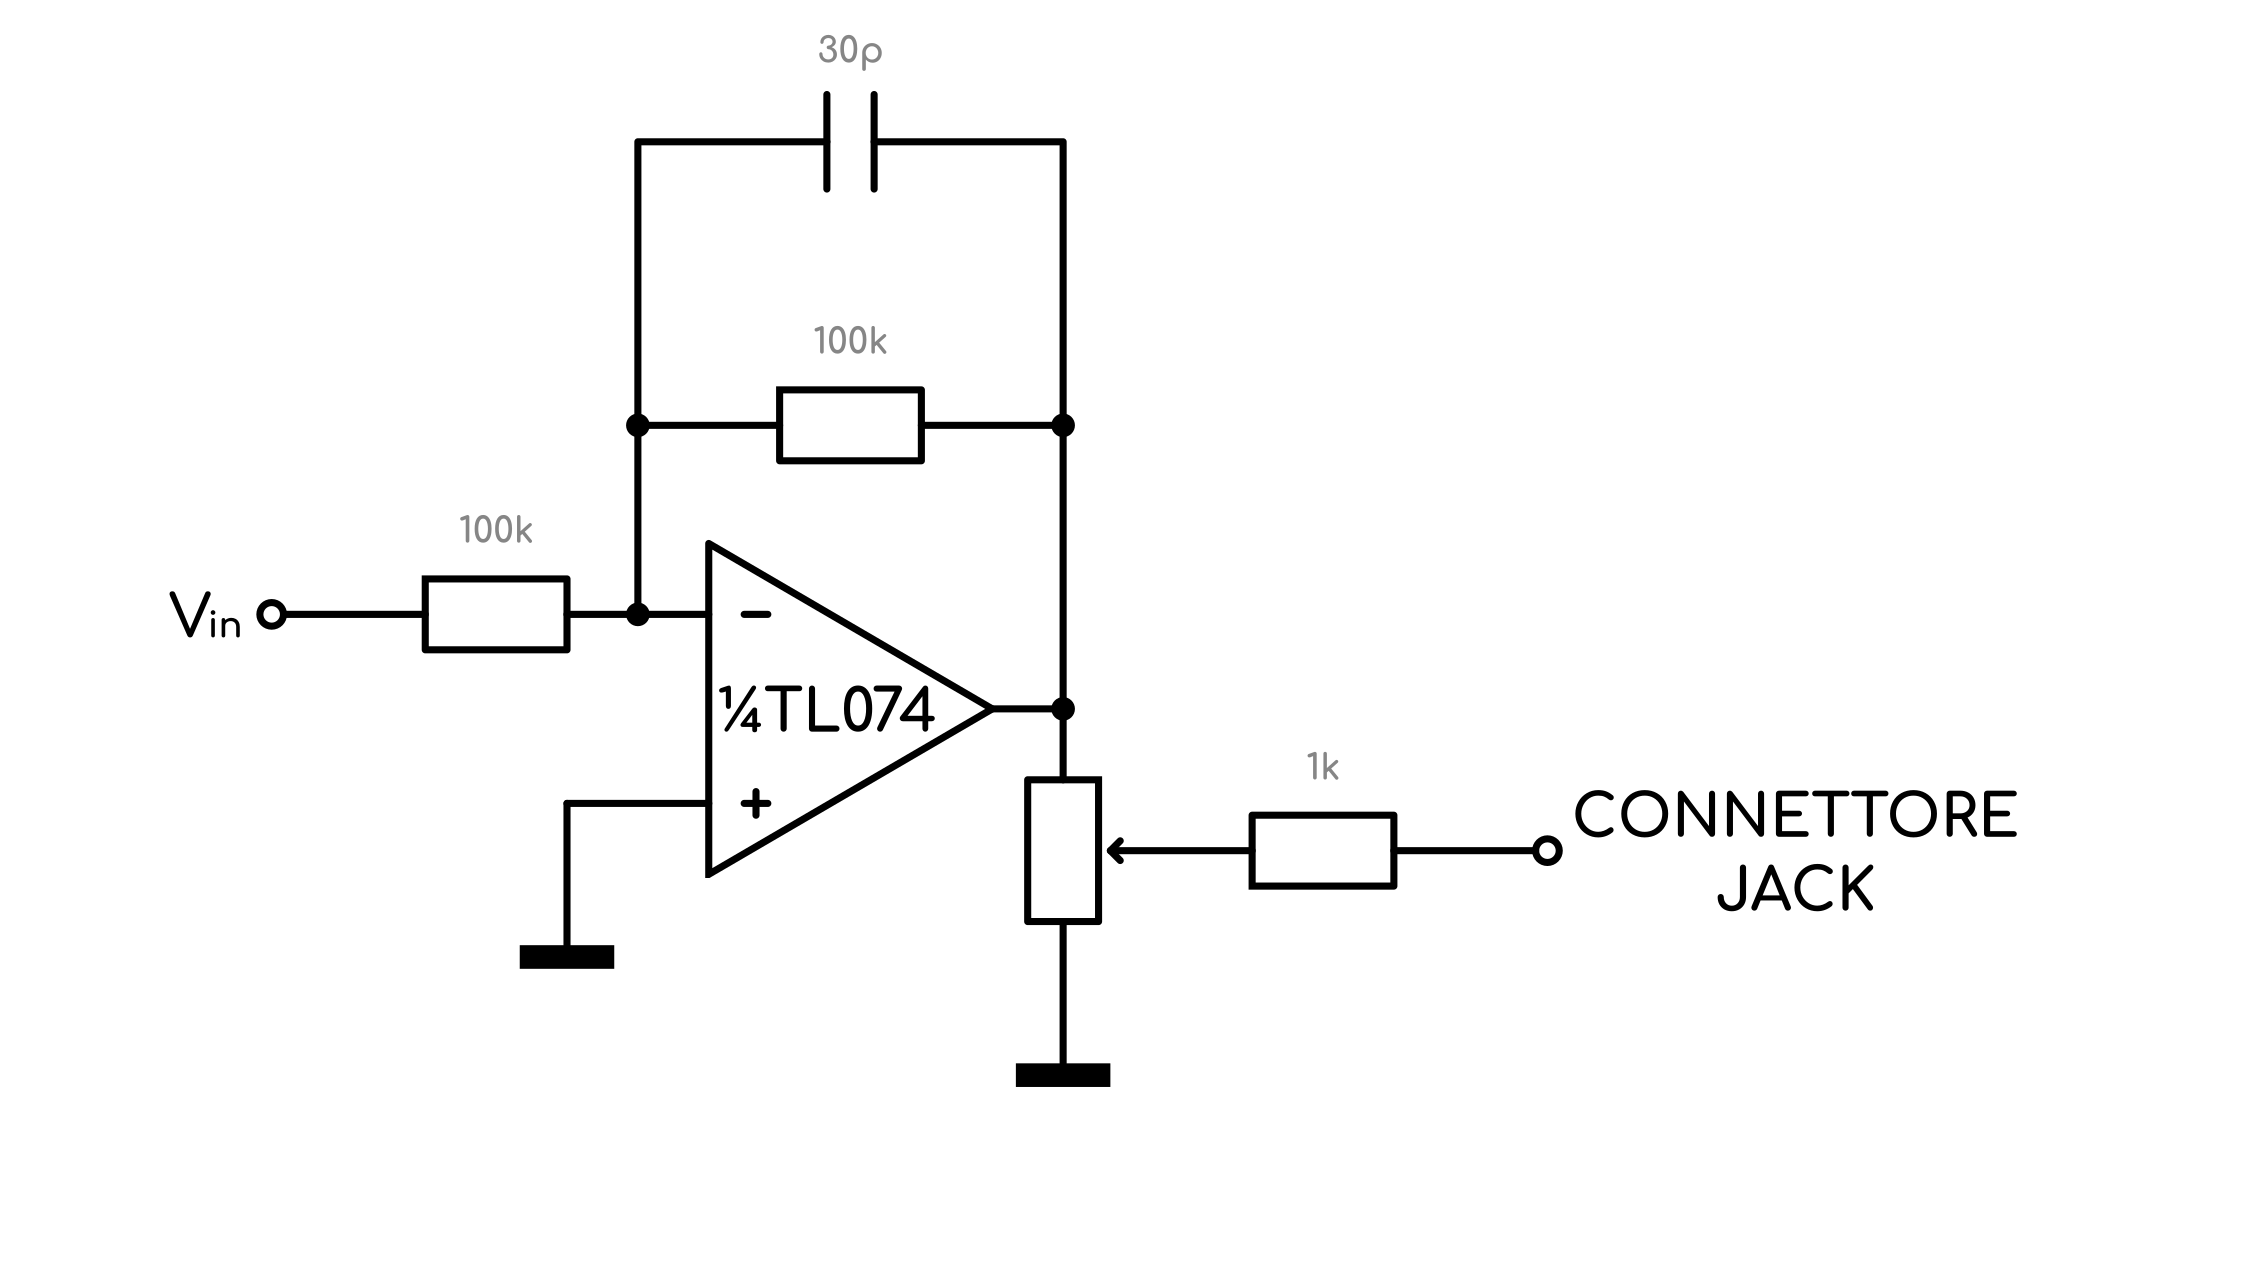
\includegraphics{circuits/inverting_output_stage_circuit.png}
        \caption{Circuito utilizzato per triangolo, sinusoide e onda quadra}
        \label{inverting_output_stage_circuit}
    \end{subfigure}
    \begin{subfigure}{\textwidth}
        \centering
        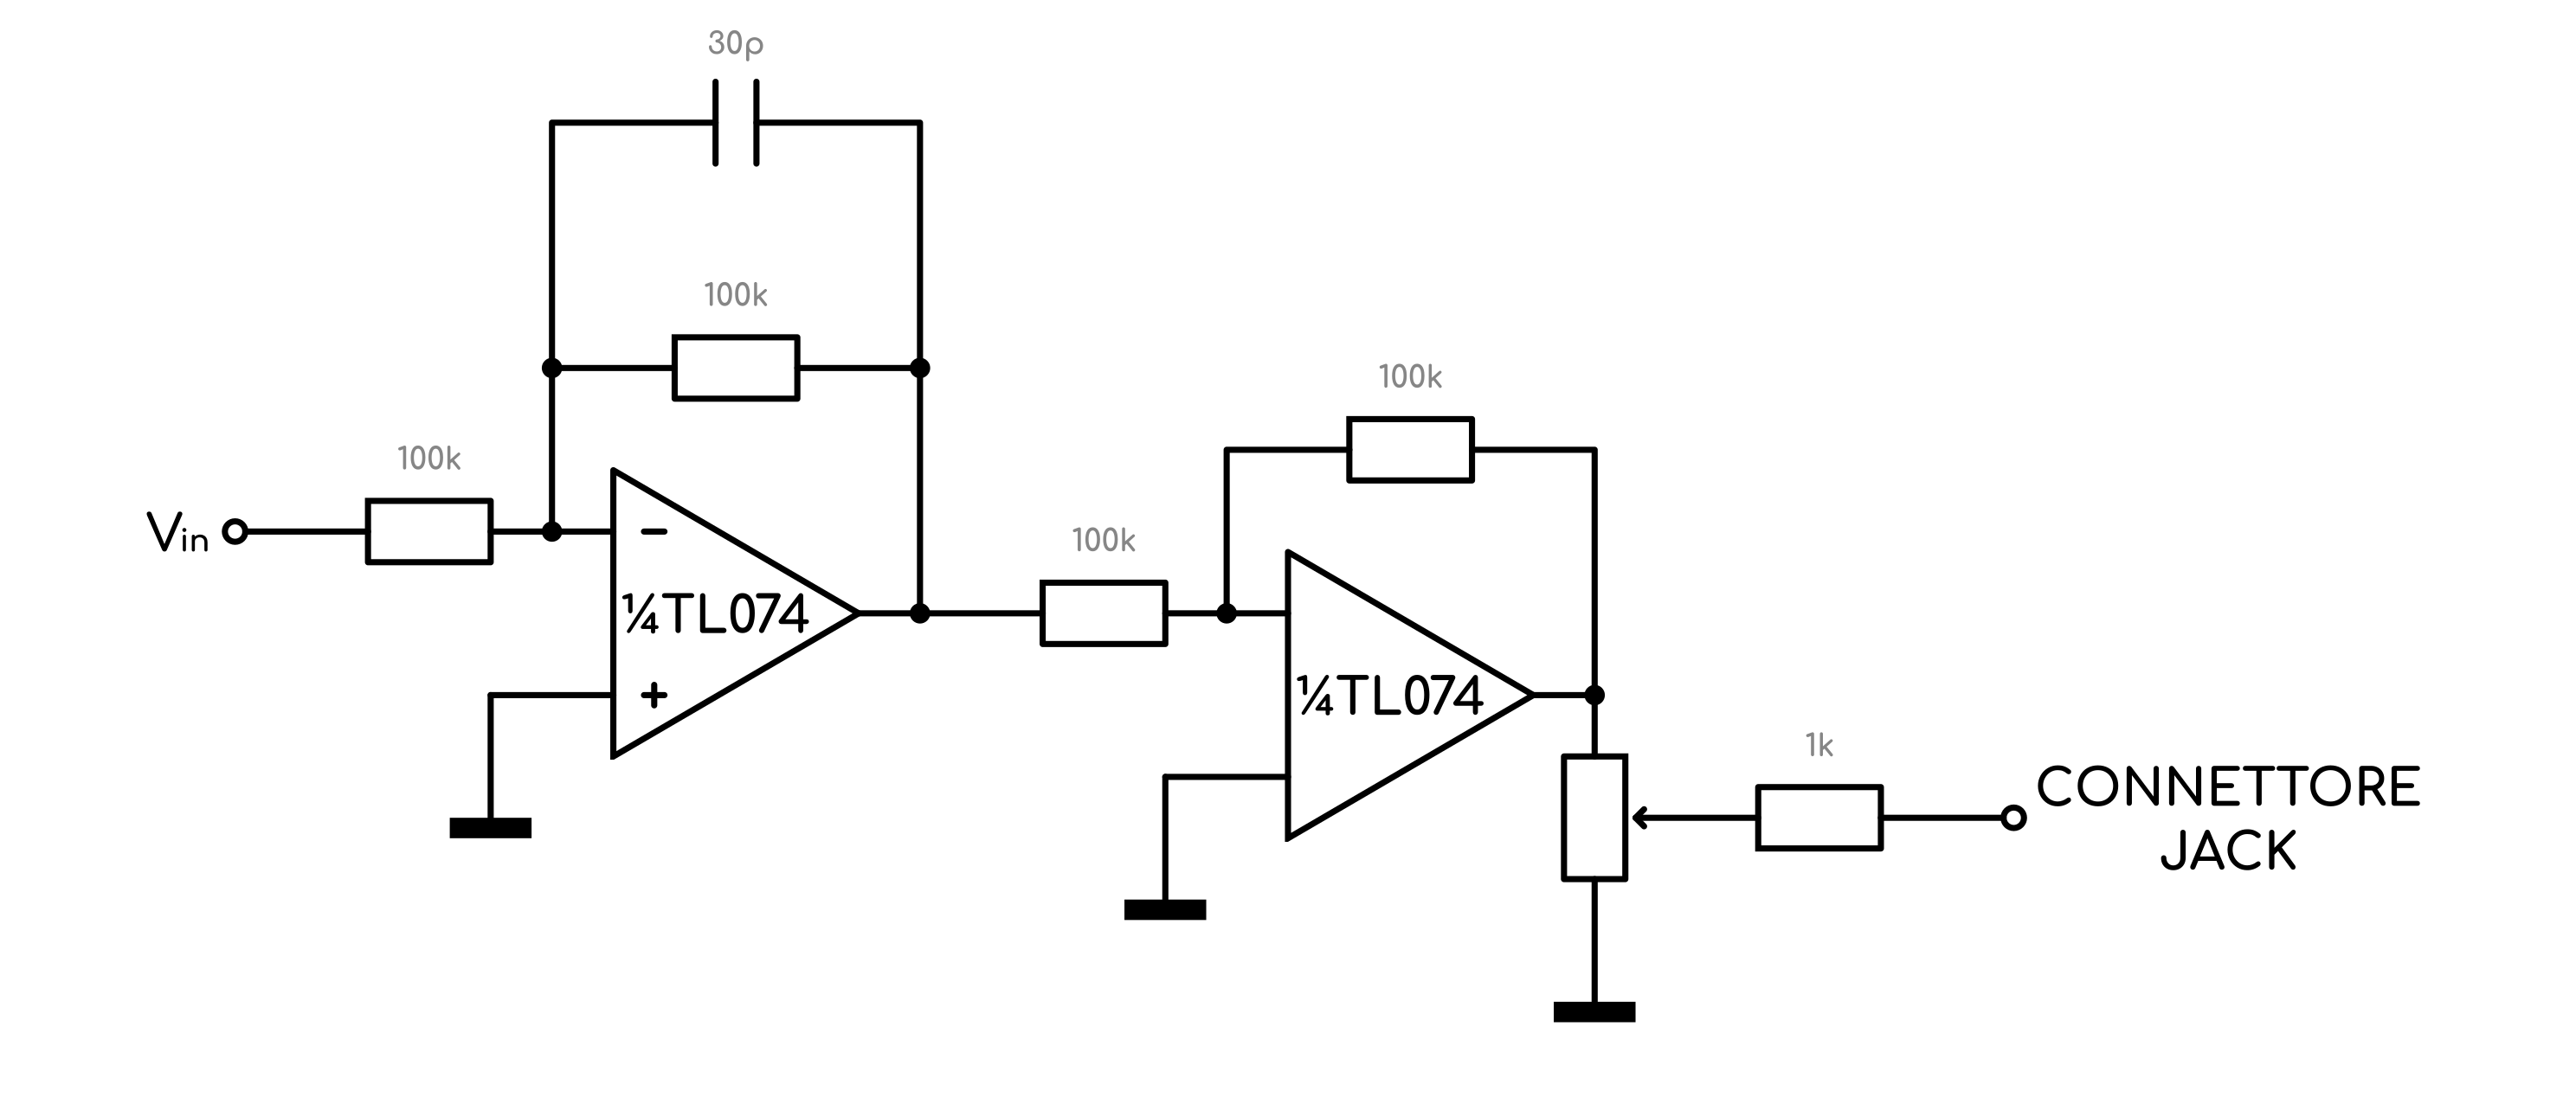
\includegraphics{circuits/noninverting_output_stage_circuit.png}
        \caption{Circuito utilizzato per rampa e dente di sega}
        \label{noninverting_output_stage_circuit}
    \end{subfigure}

    \caption{Stadi d'uscita completi}
    \label{output_stages}
\end{figure}

%--------------------------------------------------------------------------------------------
